\documentclass[uplatex,12pt,dvipdfmx]{jsarticle}

\usepackage{fullpage}
\usepackage{amsmath, amssymb, amsthm}
\usepackage{mathtools}
\usepackage{stmaryrd}

\usepackage[unicode,pagebackref]{hyperref} 
\usepackage{url}
\hypersetup{breaklinks=true}

\usepackage[all]{xy}

\usepackage{tikz}
\usetikzlibrary{matrix}
\usepackage{dynkin-diagrams}

\usepackage{empheq}


\makeatletter
\def\lst@lettertrue{\let\lst@ifletter\iffalse}
\makeatother


\setcounter{MaxMatrixCols}{20}

\theoremstyle{definition}
\newtheorem{definition}{Definition}[section]
\newtheorem{theorem}[definition]{Theorem}
\newtheorem{proposition}[definition]{Proposition}
\newtheorem{lemma}[definition]{Lemma}
\newtheorem{remark}[definition]{Remark}
\newtheorem{example}[definition]{Example}
\newtheorem{main}[definition]{Main Theorem}
\newtheorem{question}[definition]{Question}

\numberwithin{equation}{section}

\newcounter{proofcounter}[definition]

\makeatletter
\renewenvironment{proof}[1][Proof.]{\par
	\pushQED{\qed}%
	\normalfont \topsep6\p@\@plus6\p@\relax
	\trivlist
	\refstepcounter{proofcounter} %proof環境用カウンタをインクリメント
	\item[\hskip\labelsep
	\bfseries
	#1\@addpunct{.}]\ignorespaces
}{%
	\popQED\endtrivlist\@endpefalse
}


\usepackage{tcolorbox}
\tcbuselibrary{breakable} % ページまたぎに対応させる
% "myquote" という新しい環境を定義
\newtcolorbox{myquote}{
    colback=gray!10!white,
    colframe=gray!60!black,
    boxrule=0pt,   % ★先に全体の枠をなしにする
    leftrule=3mm,  % ★そのあとで左だけ太くする
    arc=0mm,
    top=1mm, bottom=1mm, left=2mm, right=2mm,
    breakable,
    parbox=false,
    after skip=1em % 箱の下の余白(あると綺麗です)
}


\newcommand{\Z}{\mathbb{Z}}
\newcommand{\Real}{\mathbb{R}}
\newcommand{\Complex}{\mathbb{C}}
\newcommand{\Projective}{\mathbb{P}}
\newcommand{\Affine}{\mathbb{A}}
\DeclareMathOperator{\linearspan}{span}
\newcommand{\Vect}{\mathrm{Vect}}
\newcommand{\Rep}{\mathrm{Rep}}
\DeclareMathOperator{\Image}{Im}
\DeclareMathOperator{\Kernel}{Ker}
\DeclareMathOperator{\length}{\ell}
\DeclareMathOperator{\Sym}{Sym}
\DeclareMathOperator{\rank}{rank}
\DeclareMathOperator{\Spec}{Spec}
\DeclarePairedDelimiter{\abra}{\langle}{\rangle} % < > angle brackets
\DeclarePairedDelimiter{\abs}{\lvert}{\rvert} % | | absolute value
\DeclarePairedDelimiter{\rbra}{\lparen}{\rparen} % () round brackets
\DeclarePairedDelimiter{\cbra}{\lbrace}{\rbrace} % {} curly brackets
\DeclarePairedDelimiter{\ssbra}{\llbracket}{\rrbracket} % [[]] double square brackets
\newcommand{\Eulercharacteristic}{\chi}
\newcommand{\Chernclass}{c}
\DeclareMathOperator{\Picard}{Pic}

\newcommand{\numGrothendieckgrp}[1]{K({#1})_{\mathrm{num}}}%numerical Grothendieck group
\newcommand{\transpose}[1]{{\vphantom{#1}}^t \hspace{-1pt}#1}


\allowdisplaybreaks

\newcommand{\Hline}[1]{\noalign{\hrule height #1}}

\newcommand{\relmiddle}[1]{\mathrel{}\middle#1\mathrel{}}

\title{}
\date{\empty}
\author{}


\begin{document}

\maketitle

\tableofcontents

\section{Markov 方程式}

\cite{devolcsey2016analoguemarkovequationexceptional}で次の Serre lattice が定義されている。

\begin{definition}
	Serre lattice $(K, \abra{\text{--}, \text{--}}, s)$とは、
	\begin{itemize}
		\item $K$: free abelian group of finite rank, 
		\item $\abra{\text{--}, \text{--}}$: $K$上のnondegenerate bilinear form, 
		\item $s$: $K$上のautomorphism
	\end{itemize}
	の組であり、
	\begin{align}
		\forall u, v\in K, \abra{u, v}=\abra{v, su}
	\end{align}
	が成り立つもののことをいう。
\end{definition}

$X$ を smooth projective threefold, $\numGrothendieckgrp{X}$ をその numerical Grothendieck group, $s$ を Serre functor が誘導する $\numGrothendieckgrp{X}$ 上の automorphism とする。
このとき $\numGrothendieckgrp{X}$ は Euler form から誘導される nondegenerate bilinear form $\abra{\text{--}, \text{--}}$ と Serre functor から誘導される $\numGrothendieckgrp{X}$ 上の automorphism $s$ を備えた Serre lattice となる。

また、{\cite[Proposition 2.1]{devolcsey2016analoguemarkovequationexceptional}}から
\begin{align}
	(s + 1)^4 = ((-1)^3 s - 1)^{3 + 1}=0
\end{align}
が成立する。

$K$ は rank $n$ の Serre lattice であるとする。
$K$ の $\Z$-basis $(e_i)_{i=1}^n$ に対して Gram matrix
\begin{align}
	M=\begin{pmatrix}
		\abra{e_1, e_1}&\cdots&\abra{e_1, e_n}\\
		\cdots&\cdots&\cdots\\
		\abra{e_n, e_1}&\cdots&\abra{e_n, e_n}
	\end{pmatrix}\in M_n(\Z)
\end{align}
を考える。
$s$ の行列表示 $S$ を
\begin{align}
	\begin{pmatrix}
		se_1&\cdots&se_n
	\end{pmatrix}=\begin{pmatrix}
		e_1&\cdots&e_n
	\end{pmatrix}S
\end{align}
で定めると
\begin{align}
	S=M^{-1}\transpose{M}
\end{align}
が成立する。

$n=4$ で $(e_i)_{i=1}^4$ が exceptional basis, つまり $M$ が対角成分1の上三角行列である場合を考える。
\begin{align}
	M = \begin{pmatrix}
		1&a&b&c\\
		0&1&d&e\\
		0&0&1&f\\
		0&0&0&1
	\end{pmatrix}\in M_4(\Z)
\end{align}
とおく。
このとき{\cite[Lem 3.1.3]{devolcsey2016analoguemarkovequationexceptional}}の類似で次が成立する。
\begin{proposition}
	\begin{gather}
		q_1(M) = acdf - abd - ace - bcf - def + a^2 + b^2 + c^2 + d^2 + e^2 + f^2, \\
		q_2(M) = af - be + cd
	\end{gather}
	とおくとき、
	\begin{align}
		(s + 1)^4 = 0
	\end{align}
	が成り立つための必要十分条件は $M$ が次のディオファントス方程式の解であることである。
	\begin{subequations}\label{markov_eq}
		\begin{empheq}[left = {\empheqlbrace \, }, right = {}]{align}
			& q_1(M) = 8\\
			& q_2(M)^2 = 16
		\end{empheq}.
	\end{subequations}
\end{proposition}

\begin{proof}
	$S$ の固有多項式 $\chi(t) = \det(tI - S)$ を考える。
	\begin{align}
		\chi(t) = \det(tI - S) = \det(tI - M^{-1}\transpose{M}) = (\det M^{-1})\det(tM - \transpose{M}) = \det(tM - \transpose{M}).
	\end{align}
	
	手計算等で
	\begin{align}
		\det(tM - \transpose{M}) = t^4 + (q_1(M) - 4)t^3 + (q_2(M)^2 - 2q_1(M) + 6)t^2 + (q_1(M) - 4)t + 1
	\end{align}
	が分かるので
	\begin{align}
		(s + 1)^4 = 0\iff&\chi(t) = (t + 1)^4\\
		\iff&q_1(M) - 4 = 4, q_2(M)^2 - 2q_1(M) + 6 = 6\\
		\iff&q_1(M) = 8, q_2(M)^2 = 16.
	\end{align}
\end{proof}

このことから$X$上に長さ4の例外生成列があれば、そのEuler formに関するGram matrixがディオファントス方程式\eqref{markov_eq}の解となることが分かる。

\section{Exceptional basis全体への作用}

$B_n$ を $n$ 本の紐に関する組み紐群、 $\sigma_1,\ldots,\sigma_{n-1}$ を $B_n$ の基本生成系とする。

$X$ 上に長さ $n$ の例外生成列があるとき、 $i=1,\ldots,n-1$ に対して $\sigma_i$ は $i$, $i+1$ 番目の成分に対するleft mutationとして例外生成列全体に作用する。
$\numGrothendieckgrp{X}$ 上では、 $X$ 上の例外生成列 $(\mathcal{E}_1,\ldots,\mathcal{E}_n)$, $i=1,\ldots,n-1$ に対して
\begin{align}
	\sigma_i\cdot(e_1,\ldots,e_n) = (e_1,\ldots,e_{i-1}, \abra{e_i, e_{i+1}}e_i - e_{i+1}, e_i, e_{i+2},\ldots,e_n)
\end{align}
という作用になる。
ただし $e_i$ は $\mathcal{E}_i$ の $\numGrothendieckgrp{X}$ での像を表す。
これを一般化し、 $B_n$ の Serre lattice の exceptional basis 全体への作用の定義として採用する。
\footnote{\cite{devolcsey2016analoguemarkovequationexceptional}や\cite{MR2084561}では符号が異なり
\begin{align}
	\sigma_i\cdot(e_1,\ldots,e_n) = (e_1,\ldots,e_{i-1}, e_{i+1} - \abra{e_i, e_{i+1}}e_i, e_i, e_{i+2},\ldots,e_n)
\end{align}
で定義している。
このあと見る $q_2$ の符号に関する命題との兼ね合いから、この定義は採用しない。
}
この作用により、exceptional basis から作られる Gram matrix にも $B_n$ の作用が反映される。
$K$ のexceptional basis $(e_1,\ldots,e_n)$ に関する Gram matrix を $M$ とするとき、 $\sigma\in B_n$ に対して $\sigma\cdots(e_1,\ldots,e_n)$ に関する Gram matrix を$\sigma\cdot M$とかくことにする。

$i=1,\ldots,n-1$, $m\in\Z$ に対して
\begin{equation}
	A_j(m)=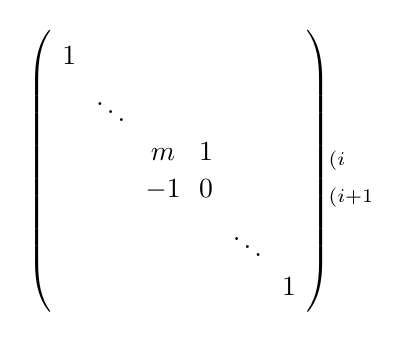
\begin{tikzpicture}[%
		baseline=(m.west),
		every left delimiter/.style={xshift=1ex},
		every right delimiter/.style={xshift=-1ex}]
		\matrix(m)[matrix of math nodes,nodes in empty cells,
		left delimiter={(},right delimiter={)}]
		{
			1 &  &  &  &  &  \\
			& \ddots &  &  &  &  \\
			&  & m & 1 &  &  \\
			&  & -1 & 0 &  &  \\
			&  &  &  & \ddots &  \\
			&  &  &  &  & 1\\
		};
		\node[right=2.5ex]at(m-3-6){${\scriptstyle(i}$};
		\node[right=2.5ex]at(m-4-6){${\scriptstyle(i+1}$};
	\end{tikzpicture}
\end{equation}
と定めるとき、$\forall i=1,\ldots,n-1$ に対して $(e^\prime_1,\ldots,e^\prime_n)=\sigma_i\cdot(e_1,\ldots,e_n)$ とおくと、
\begin{align}
	\begin{pmatrix}
		e^\prime_1&\cdots&e^\prime_n
	\end{pmatrix}=\begin{pmatrix}
		e_1&\cdots&e_n
	\end{pmatrix}A_i(\abra{e_i, e_{i+1}})
\end{align}
が成り立つので
\begin{align}
	\sigma_i\cdot M = \transpose{A_i(\abra{e_i, e_{i+1}})} M A_i(\abra{e_i, e_{i+1}})
\end{align}
という関係が成立する。

$n=4$ の場合を具体的に計算すると次の通り:
\begin{gather}
	\sigma_1 \cdot M = \begin{pmatrix}
		1 & a & ab-d & ac-e \\
		0 & 1 & b & c \\
		0 & 0 & 1 & f \\
		0 & 0 & 0 & 1
	\end{pmatrix},\\
	\sigma_2 \cdot M = \begin{pmatrix}
		1 & ad-b & a & c \\
		0 & 1 & d & de-f \\
		0 & 0 & 1 & e \\
		0 & 0 & 0 & 1
	\end{pmatrix},\\
	\sigma_3 \cdot M = \begin{pmatrix}
		1 & a & fb-c & b \\
		0 & 1 & fd-e & d \\
		0 & 0 & 1 & f \\
		0 & 0 & 0 & 1
	\end{pmatrix}.
\end{gather}

$X$ 上の例外生成列には $\Z^n$ の作用も定義できる。
$\epsilon_1,\ldots,\epsilon_n$ を $\Z^n$ の標準基底とするとき、$X$ 上の例外生成列 $(\mathcal{E}_1,\ldots,\mathcal{E}_n)$, $i=1,\ldots,n-1$ に対して
\[ \epsilon_i\cdot(\mathcal{E}_1,\ldots,\mathcal{E}_n)=(\mathcal{E}_1,\ldots,\mathcal{E}_{i-1},\mathcal{E}_i[1],\mathcal{E}_{i+1},\ldots,\mathcal{E}_n) \]
という作用になる。

$\numGrothendieckgrp{X}$ 上では shift functor は $(-1)$ 倍することに対応し、
\begin{align}
	\epsilon_i\cdot(e_1,\ldots,e_n) = (e_1,\ldots,e_{i-1}, -e_i, e_{i+1},\ldots,e_n)
\end{align}
という作用になる。
ただし $e_i$ は $\mathcal{E}_i$ の $\numGrothendieckgrp{X}$ での像を表す。
これを一般化し、$\Z^n$ の Serre lattice の exceptional basis 全体への作用の定義として採用する。
\footnote{本質的には $(\Z/2\Z)^n$ の作用となる。}
この作用により、exceptional basis から作られる Gram matrix にも $\Z^n$ の作用が反映される。
$K$ の exceptional basis $(e_1,\ldots,e_n)$ に関する Gram matrix を $M$ とするとき、$v\in B_n$ に対して $v\cdot(e_1,\ldots,e_n)$ に関する Gram matrix を $v\cdot M$ とかくことにする。

$n=4$ の場合を具体的に計算すると次の通り:
\begin{gather}
	\epsilon_1 \cdot M = \begin{pmatrix}
		1 & -a & -b & -c \\
		0 & 1 & d & e \\
		0 & 0 & 1 & f \\
		0 & 0 & 0 & 1
	\end{pmatrix},\\
	\epsilon_2 \cdot M = \begin{pmatrix}
		1 & -a & b & c \\
		0 & 1 & -d & -e \\
		0 & 0 & 1 & f \\
		0 & 0 & 0 & 1
	\end{pmatrix},\\
	\epsilon_3 \cdot M = \begin{pmatrix}
		1 & a & -b & c \\
		0 & 1 & -d & e \\
		0 & 0 & 1 & -f \\
		0 & 0 & 0 & 1
	\end{pmatrix},\\
	\epsilon_4 \cdot M = \begin{pmatrix}
		1 & a & b & -c \\
		0 & 1 & d & -e \\
		0 & 0 & 1 & -f \\
		0 & 0 & 0 & 1
	\end{pmatrix}.
\end{gather}

以上で $B_n\ltimes\Z^n$ の作用が定義された。

$n=4$ で $(s + 1)^4 = 0$ が成立する場合は $\forall\sigma\in B_4\ltimes\Z^4$ に対して $\sigma\cdot M$ もディオファントス方程式\eqref{markov_eq}の解となる。
このうち、$q_2$ については $4,-4$ の 2 通りの値を取り得るが、 $B_n$ の作用では $q_2$ は保存される。
一方、$\epsilon_1,\epsilon_2,\epsilon_3,\epsilon_4$ の作用では符号が反転する。

\begin{proposition}
	$K$ は Serre lattice of rank $4$ であるとする。
	このとき $\forall\sigma\in B_n$ について
	\begin{align*}
		q_2(\sigma\cdot M) = q_2(M)
	\end{align*}
	が成立する。
\end{proposition}

\begin{proof}
	手計算で $\sigma_1\cdot M,\sigma_2\cdot M,\sigma_3\cdot M$ について成立することが分かる。
\end{proof}

\begin{proposition}
	$K$ は Serre lattice of rank $4$ であるとする。
	このとき $\forall i=1,2,3,4$ について
	\begin{align*}
		q_2(\epsilon_i\cdot M) = -q_2(M)
	\end{align*}
	が成立する。
\end{proposition}

\begin{proof}
	手計算で成立することが分かる。
\end{proof}


以上でディオファントス方程式\eqref{markov_eq}の解に対する $B_4\ltimes\Z^4$ の作用が定義された。

\section{4つのthreefold}

{\cite[Lemma 3.5]{nordskova2025exceptionalcollectionsfanothreefolds}}によると 4 つのベクトル束からなる例外生成列を持つ smooth projective threefold は $X = \Projective^3,Q_3,V_5,V_{22}$ に限られる。
これらの例外生成列からディオファントス方程式\eqref{markov_eq}の解の系列が得られる。
例外生成列をひとつ列挙し、その系列の代表系となるGram matrixを計算する。

\subsection{$\Projective^3$}

\cite{MR509388}で $(\mathcal{O}_{\Projective^n}, \mathcal{O}_{\Projective^n}(1), \ldots, \mathcal{O}_{\Projective^n}(n))$ は $\Projective^n$ の例外生成列であることが示されている。
特に $(\mathcal{O}_{\Projective^3}, \mathcal{O}_{\Projective^3}(1), \mathcal{O}_{\Projective^3}(2), \mathcal{O}_{\Projective^3}(3))$ は $\Projective^3$ の例外生成列となる。
Gram matrixは
\begin{gather}
	M_{\mathbb{P}^3} = \begin{pmatrix}
		1 & 4 & 10 & 20 \\
		0 & 1 & 4 & 10 \\
		0 & 0 & 1 & 4 \\
		0 & 0 & 0 & 1
	\end{pmatrix},\\
	q_2(M_{\mathbb{P}^3}) = -4
\end{gather}
となる。

\subsection{$Q_3$}

$\Projective^{n+1}$ 内の $2$ 次超曲面を$Q_n$とかく。
$n$が奇数のとき、$n = 2k + 1$ とおくと、$Q_n$は$B_{k+1}$型の単連結複素単純 Lie 群 $G = Spin(2k + 3)$ の旗多様体とみなせる。
対応する crossed out Dynkin diagram は $\dynkin[labels={\alpha_1,,,\alpha_{k+1}}] B{x*...**}$となる。

最高ウェイトが$(0,\ldots,0,1)$\footnote{メモ:小林さんのパッケージでの最高ウェイト}である$Q_n$上の同変ベクトル束を$\Sigma$とかくことにする。
$\Sigma$はスピノル束と呼ばれている。
このとき $(\mathcal{O}_{Q_3}(-2), \mathcal{O}_{Q_3}(-1), \mathcal{O}_{Q_3}, \Sigma)$ は $Q_3$ の例外生成列であることが\cite{MR939472}で示されている。
\footnote{メモ:\cite{ABondal1995SemiorthogonalDF}でもそのように引用されている。}
Gram matrixは
\begin{gather}
	M_{Q_3} = \begin{pmatrix}
		1 & \Eulercharacteristic(\mathcal{O}_{Q_3}(1)) & \Eulercharacteristic(\mathcal{O}_{Q_3}(2)) & \Eulercharacteristic(\Sigma(2)) \\
		0 & 1 & \Eulercharacteristic(\mathcal{O}_{Q_3}(1)) & \Eulercharacteristic(\Sigma(1)) \\
		0 & 0 & 1 & \Eulercharacteristic(\Sigma) \\
		0 & 0 & 0 & 1
	\end{pmatrix} = \begin{pmatrix}
		1 & 5 & 14 & 40 \\
		0 & 1 & 5 & 16 \\
		0 & 0 & 1 & 4 \\
		0 & 0 & 0 & 1
	\end{pmatrix},\\
	q_2(M_{Q_3}) = -4
\end{gather}
となる。
\footnote{$\mathcal{O}_{Q_3}(1)$ が最高ウェイト $(1, 0)$ に対応し、$\mathcal{O}_{Q_3}(2)$, $\Sigma$, $\Sigma(1)$, $\Sigma(2)$ もそれぞれ $(2, 0)$, $(0, 1)$, $(1, 1)$, $(2, 1)$ に対応する。
小林さんパッケージ(を少し修正したもの)で計算してみた結果となる。
Geminiの主張とも一致する。}


\subsection{$V_5$}

$V_5$ とは、Grassmann 多様体 $Gr(2,5)$ の一般的な 3 つの超平面により切り取られる断面として実現される Fano threefold である。

$Gr(2,5)$ は $A_4$型の $SL(5,\Complex)$ の旗多様体であり、対応する crossed out Dynkin diagram は $\dynkin[labels={\alpha_1,\alpha_2,\alpha_3,\alpha_4}] A{*x**}$となる。
$\mathcal{U}$ を $Gr(2,5)$ 上の tautological bundle を $V_5$ に制限したものとする。
このとき $(\mathcal{O}_{V_5}, \mathcal{U}^*, \mathcal{O}_{V_5}(1), \mathcal{U}^*(1))$ は $V_5$ の例外生成列であることが\cite{MR1294662}で示されている。
Gram matrixは
\begin{gather}
	M_{V_5} = \begin{pmatrix}
		1 & \Eulercharacteristic(\mathcal{U}^*) & \Eulercharacteristic(\mathcal{O}_{V_5}(1)) & \Eulercharacteristic(\mathcal{U}^*(1)) \\
		0 & 1 & \Eulercharacteristic(\mathcal{U}(1)) & \Eulercharacteristic(\mathcal{U}\otimes\mathcal{U}^*(1)) \\
		0 & 0 & 1 & \Eulercharacteristic(\mathcal{U}^*) \\
		0 & 0 & 0 & 1
	\end{pmatrix} = \begin{pmatrix}
		1 & 5 & 7 & 25 \\
		0 & 1 & 5 & 22 \\
		0 & 0 & 1 & 5 \\
		0 & 0 & 0 & 1
	\end{pmatrix},\\
	q_2(M_{V_5}) = -4
\end{gather}
となる。
\footnote{$\mathcal{O}_{V_5}(1)$ が最高ウェイト $(0, 1, 0, 0)$, $\mathcal{U}^*$ が$(1, 0, 0, 0)$に対応する。
小林さんのパッケージによる計算結果であり、Geminiの主張とも一致する。}

\subsection{$V_{22}$}

$V_{22}$ とは、$Gr(3, 7)$ 上の tautological bundle を $\mathcal{U}$ とするとき、$(\bigwedge^2 \mathcal{U}^\vee)^{\oplus3}$の一般切断として実現される Fano threefold である。

$Gr(3,7)$ は $A_6$型の $SL(7,\Complex)$ の旗多様体であり、対応する crossed out Dynkin diagram は $\dynkin[labels={\alpha_1,\alpha_2,\alpha_3,\alpha_4,\alpha_5,\alpha_6}] A{**x***}$となる。
このとき rank $2$のベクトル束$\mathcal{E}$
\footnote{Mukai bundleとよばれている。
	$V_{22}$ の超平面切断 $Y$ 上の直線束 $\mathcal{O}_Y(L)$ に付随して定義される束で、以下の完全列を満たす核として定義される。
	\begin{align}
		\xymatrix{
			0 \ar[r] &\mathcal{E} \ar[r]& H^0(\mathcal{O}_Y(L)) \otimes \mathcal{O}_X \ar[r]& \mathcal{O}_Y(L) \ar[r]& 0
		}.
	\end{align}
	ここで $L$ は $V_{22}$ 上の直線を表す。
	また、双対束 $\mathcal{E}^\vee$ は $\mathcal{E} \otimes \mathcal{O}_X(-K_X)$ と同型になる。
}
が存在して $\mathcal{U}$ は $V_{22}$ に制限したものを意味するとして $(\mathcal{O}_{V_{22}}, \mathcal{U}^*, \mathcal{E}^*, \bigwedge^2 \mathcal{U}^*)$ は $V_{22}$ の例外生成列であることが\cite{MR1445274}で示されている。

ただし、GeminiとSageMathによる計算結果によれば$\mathcal{E}$は$K$群において
\begin{align}
	[\mathcal{E}^\vee] = -\frac{1}{20}[\mathcal{O}_{V_{22}}] + \frac{7}{20}[\mathcal{U}^*] + \frac{7}{20}[\bigwedge^2 \mathcal{U}^*] - \frac{1}{20}[\mathcal{O}_{V_{22}}(1)]
\end{align}
を満たすベクトル束らしい。
Gram matrixは
\begin{gather}
	M_{V_{22}} = \begin{pmatrix}
		1 & \Eulercharacteristic(\mathcal{U}^*) & \Eulercharacteristic(\mathcal{E}^*) & \Eulercharacteristic(\bigwedge^2 \mathcal{U}^*) \\
		0 & 1 & \Eulercharacteristic(\mathcal{U}\otimes\mathcal{E}^*) & \Eulercharacteristic(\mathcal{U}\otimes\bigwedge^2 \mathcal{U}^*) \\
		0 & 0 & 1 & \Eulercharacteristic(\mathcal{E}\otimes\bigwedge^2 \mathcal{U}^*) \\
		0 & 0 & 0 & 1
	\end{pmatrix} = \begin{pmatrix}
		1 & 7 & 8 & 18 \\
		0 & 1 & 4 & 13 \\
		0 & 0 & 1 & 4 \\
		0 & 0 & 0 & 1
	\end{pmatrix},\\
	q_2(M_{V_{22}}) = -4
\end{gather}
となる。
\footnote{$\mathcal{U}^*$ は $(1, 0, 0, 0, 0, 0)$ に対応する。}

\begin{question}
	ディオファントス方程式\eqref{markov_eq}の解の $B_n\ltimes\Z^n$ あるいは $B_n$ による orbit は $\Projective^3$, $Q_3$, $V_5$, $V_{22}$ のもので尽きるか?
	また、これらは異なる orbit を成すか?
\end{question}

\section{数値的解の探索と独立性の証明}

計算機探索により、既知の4つの多様体($\Projective^3, Q_3, V_5, V_{22}$)のいずれの軌道にも属さない数値的解(Numerical Solution)の存在が確認された。
以下にその具体例と、独立性の証明を与える。

\subsection{数値的解の発見}
成分の絶対値が小さい範囲での全探索により、多数の新しい解が見出された。
その中でも最小のノルム(非対角成分の二乗和の平方根)を持つ例として、以下の行列 $M_{\mathrm{ghost}}$ を挙げる。

\begin{align}
    M_{\mathrm{ghost}} = \begin{pmatrix}
        1 & 0 & 2 & 0 \\
        0 & 1 & 0 & 2 \\
        0 & 0 & 1 & 0 \\
        0 & 0 & 0 & 1
    \end{pmatrix}
\end{align}

この行列の不変量は $q_1(M_{\mathrm{ghost}}) = 8, q_2(M_{\mathrm{ghost}}) = 4$ であり、Markov型方程式の条件を満たす。

\subsection{別軌道であることの証明}

発見された解 $M_{\mathrm{ghost}}$ が、既知の4つの多様体の軌道 $O_{X}$ ($X \in \{\Projective^3, Q_3, V_5, V_{22}\}$) のいずれにも含まれないことを、有限体 $\mathbb{F}_3$ 上への還元を用いて証明する。

\begin{theorem}
    数値的解 $M_{\mathrm{ghost}}$ は、$\Projective^3, Q_3, V_5, V_{22}$ のいずれの $B_n\ltimes\Z^n$ 軌道にも属さない。
\end{theorem}

\begin{proof}
    もし $M_{\mathrm{ghost}}$ がある多様体 $X$ の軌道 $O_X$ に含まれるならば、任意の素数 $p$ に対して、法 $p$ で還元した行列も対応する軌道 $\overline{O_X}^{(p)}$ に含まれなければならない。
    
    $p=3$ において、各多様体の軌道全体 $\overline{O_X}^{(3)}$ を計算機により生成したところ、その要素数は以下の通りであった。
    \begin{itemize}
        \item $|\overline{O_{\Projective^3}}^{(3)}| = 216$
        \item $|\overline{O_{Q_3}}^{(3)}| = 8$
        \item $|\overline{O_{V_5}}^{(3)}| = 216$
        \item $|\overline{O_{V_{22}}}^{(3)}| = 216$
    \end{itemize}
    
    一方、$M_{\mathrm{ghost}}$ を法 $3$ で還元すると
    \begin{align}
        M_{\mathrm{ghost}} \equiv \begin{pmatrix}
            1 & 0 & 0 & 0 \\
            0 & 1 & 1 & 1 \\
            0 & 0 & 1 & 0 \\
            0 & 0 & 0 & 1
        \end{pmatrix} \pmod 3
    \end{align}
    となる。この行列は、上で生成したどの集合 $\overline{O_X}^{(3)}$ にも含まれないことが確認された。
    したがって、対偶により $M_{\mathrm{ghost}}$ は整数環 $\Z$ 上において、これら4つの多様体のどの軌道にも属さない。
\end{proof}

なお、同様の方法で他の数値的解についても独立性を確認している。

また、modulo 6での軌道の要素数から$\Projective^3, Q_3, V_5, V_{22}$の軌道が互いに異なることも確認できる。

\subsection{結論}
以上の結果より、方程式\eqref{markov_eq}の整数解の軌道は、既知のFano 3-fold由来の4つの系列だけでは尽くされないことが示された。
今回発見された数値的解は、幾何学的な背景を持たない(あるいは未知の幾何学的対象に対応する)数値的解であると考えられる。

そこで、次の問題を考える。

\begin{question}\label{question:1}
	ディオファントス方程式\eqref{markov_eq}の解の $B_n\ltimes\Z^n$ あるいは $B_n$ による orbit は無限に存在するか?
\end{question}

\begin{remark}
	\cite{MR4803470}においてStokes行列の空間の整数点に関する結果がある。
	$V_p(4)$ を Stokes行列 $S$ であって、$\det(\lambda I + S^{-1}({}^tS))$ が 多項式 $p$ に一致する空間として定義する。
	Stokes行列はこのノートで取り扱う exceptional basis に対する Gram matrix と同一視できる。
	$p$ が相反多項式であり、そのdiscriminantが非零であるとき、$V_p(4)$ の整数点の $B_4$-orbit は有限個であることが示されている。
	このノートで取り扱うケースは$p=(\lambda-1)^4$に対応し、discriminantが零であるため、この結果は適用されない。
\end{remark}

\begin{question}\label{question:2}
	ディオファントス方程式\eqref{markov_eq}の解の $B_n\ltimes\Z^n$ あるいは $B_n$ による orbit をすべて分類できるか?
\end{question}

\begin{question}\label{question:3}
	$B_n\ltimes\Z^n$よりもさらに大きい、由緒正しい群でディオファントス方程式\eqref{markov_eq}の解に作用するものは存在するか?
\end{question}

\begin{question}\label{question:4}
	発見された数値的解に対応する非可換代数幾何学的対象(圏)は構成できるか?
\end{question}

\begin{question}\label{question:5}
	数値的解に対応する非可換代数幾何学的対象(圏)の性質はどのようなものか? 例えば、これらの圏の Hochschild ホモロジーや K 群はどのような構造を持つか?
\end{question}

\begin{question}\label{question:6}
	幾何的解(ノルム $\geq 136$)と数値的解(ノルム $\leq 44$)の間には、なぜこれほど大きな断絶(ギャップ)があるのか? 中間のノルムを持つ解は存在しないのか?
	※数値的解の探索範囲がただ小さいだけと予想されるが、念のため。
\end{question}

\begin{question}\label{question:7}
	発見された数値的解において、Serre functor $S = M^{-1} {}^t M$ のJordan blockのサイズの分布に何か法則はあるか?
\end{question}

\begin{remark}
    いくつかの発見された数値的解 $M_{\mathrm{ghost}}$ について、Serre functor $S = M_{\mathrm{ghost}}^{-1} \transpose{M_{\mathrm{ghost}}}$ のJordan標準形を計算したところ、以下の2種類の異なる構造が見出された。

    \begin{enumerate}
        \item \textbf{Type [4] (Maximally Unipotent):}
        ノルムが $10, 26, 44$ などの解に見られる構造。固有値 $-1$ に対応する $4 \times 4$ のJordanブロックを一つだけ持つ。これは既知のFano 3-foldと同様の性質であり、これらは非可換Fano 3-foldの有力な候補であると考えられる。
        
        \item \textbf{Type [2, 2]:}
        ノルムが $8$ の解(最小ノルム解)に見られる構造。$2 \times 2$ のJordanブロック2つからなる。これは、対応する幾何学的対象が可約であるか、あるいは低次元の対象の積(例えば曲面と曲線の積など)のような構造を持っている可能性を示唆している。
    \end{enumerate}
\end{remark}

\begin{question}\label{question:8}
	$q_1(M) = 8, q_2(M) = -4$, あるいは $q_1(M) = 8, q_2(M) = 4$ で定義される代数多様体はrationalか?
\end{question}

\begin{question}\label{question:9}
	今回は $n=4$(Fano 3-foldに対応)を扱ったが、$n=5$ の場合に同様の「数値的解」は現れるか?
\end{question}

\begin{question}\label{question:10}
	ディオファントス方程式\eqref{markov_eq}の $\mathbb{F}_q$ における解の個数でわかることはあるか?
\end{question}


\section{$B_4$軌道は無限に存在するか?}

Question \ref{question:1} に取り組む。

★Serre operatorの$F_p$上でのJordan標準形のブロックサイズを用いれば証明できるのでは?
各$p$について、Serre operatorのJordan標準形のブロックサイズは$B_4$-invariantになると思われ、これが異なる解を無限に構成できることを示せば良い。
示せばいいがこれが大変そう。


\section{$q_1(M) = 8, q_2(M) = -4$ で定まる代数多様体はrationalか?}

\subsection{試行錯誤}

Question \ref{question:8} に取り組む。
もし rational なら、$q_1(M) = 8, q_2(M) = -4$ の一般的な有理数解を媒介変数を用いて表示できることになる。
$q_1(M) = 8, q_2(M) = -4$ で定まる$\Affine^6$ 内の代数多様体 $X$ に対する birational な式変形を試みる。

$af - be + cd = q_2(M) = -4$ から $a\neq0$の open subset 上で考えると
\begin{align}
	f = \frac{be - cd - 4}{a}
\end{align}
となり、これを
\begin{align}
	acdf - abd - ace - bcf - def + a^2 + b^2 + c^2 + d^2 + e^2 + f^2 = q_1(M) = 8
\end{align}
に代入する。
そのあと $a^2$ 倍して分母を払って整理すると次が得られる。
\begin{equation}
	\begin{aligned}[t]
		& a^4 - a^3bd - a^3ce + a^2b^2 + a^2bcde - a^2c^2d^2 + a^2c^2 - 4a^2cd + a^2d^2 + a^2e^2\\
		& - 8a^2 - ab^2ce + abc^2d + 4abc - abde^2 + acd^2e + 4ade + b^2e^2 - 2bcde\\
		& - 8be + c^2d^2 + 8cd + 16 = 0.
	\end{aligned}
\end{equation}

$e$ に注目すると、$e$ の2次式になっていて、
\begin{gather}
	A = a^2 - abd + b^2,\\
	B = -a^3c + a^2bcd - ab^2c + acd^2 + 4ad - 2bcd - 8b,\\
	C = a^4 - a^3bd + a^2b^2 - a^2c^2d^2 + a^2c^2 - 4a^2cd + a^2d^2 - 8a^2 + abc^2d + 4abc + c^2d^2 + 8cd + 16
\end{gather}
とおいて
\begin{align}
	Ae^2 + Be + C = 0
\end{align}
と書ける。
最後の式を平方完成して、
\begin{gather}
	\rbra*{2Ae + B}^2 = B^2 - 4AC.
\end{gather}
よって
\begin{gather}
	w = 2Ae + B,\\
	\Delta = B^2 -4AC
\end{gather}
とおけば $X$ は $\Affine^5$内で
\begin{align*}
	w^2 = \Delta(a,b,c,d)
\end{align*}
で定義される超曲面と birational となる。
計算機での計算結果で
\begin{equation}
	\begin{aligned}
		\Delta/a^2 = & a^4c^2 - 4a^4 - 2a^3bc^2d + 8a^3bd + a^2b^2c^2d^2 + 2a^2b^2c^2  \\
		& - 4a^2b^2d^2 - 8a^2b^2 + 2a^2c^2d^2 - 4a^2c^2 + 8a^2cd - 4a^2d^2 + 32a^2  \\
		& - 2ab^3c^2d + 8ab^3d - 2abc^2d^3 + 4abc^2d - 8abcd^2 + 4abd^3 - 32abd  \\
		& + b^4c^2 - 4b^4 + 2b^2c^2d^2 - 4b^2c^2 + 8b^2cd - 4b^2d^2 + 32b^2  \\
		& + c^2d^4 - 4c^2d^2 + 8cd^3 - 32cd + 16d^2 - 64 
	\end{aligned}
\end{equation}
となり、$\Delta$ は$a^2$で割り切れる。
\begin{align}
	\Delta_0 = \Delta/a^2
\end{align}
とすれば $X$ は $\Affine^5$ 内で
\begin{align}
	w^2 = \Delta_0(a,b,c,d)
\end{align}
で定義される超曲面 と birational となる。

$\Delta_0$ は $d$ について2次式になっている。
実は
\begin{gather}
	D = A + d^2 - 4 = a^2 - abd + b^2 + d^2 - 4,\\
	E = D(c^2 - 4) + 4(d + c)^2
\end{gather}
とおくと、計算機での計算結果で
\begin{align}
	\Delta_0 = DE
\end{align}
が分かる。
よって
\begin{align}
	w^2 = DE = D^2(c^2 - 4) + 4D(d + c)^2.
\end{align}
そこで $D\neq0$ で
\begin{align}
	u=\frac{w}{D}
\end{align}
と取れば
\begin{align}
	u^2 = (c^2 - 4) + \frac{4(d + c)^2}{D}
\end{align}
となり、
\begin{align}
	D(u^2 - c^2 + 4) = 4(d + c)^2
\end{align}
となる。
$D$ を戻して $d$ について整理すると
\begin{gather}
	S = u^2 - c^2,\\
	T = -ab(u^2 - c^2 + 4) -8c ,\\
	U = (a^2 + b^2 - 4)(u^2 - c^2 + 4) - 4c^2
\end{gather}
とおいて
\begin{align}
	Sd^2 + Td + U = 0.
\end{align}
平方完成して
\begin{align}
	\rbra*{2Sd + T}^2 = T^2 - 4SU.
\end{align}
以前と同じように
\begin{gather}
	v = 2Sd + T,\\
	\Delta_2 = T^2 - 4SU
\end{gather}
として
\begin{align}
	v^2 = \Delta_2(a,b,c,u)
\end{align}
が得られた。
$\Delta_2$は
\begin{align}
	K = u^2 - c^2 + 4
\end{align}
を因子に持ち、
\begin{align}
	\Delta_2 = K((a^2-4)(b^2-4)K + 16(a^2+b^2+c^2+abc-4))
\end{align}
となる。
\begin{gather}
	\lambda = \frac{v}{K},\\
	C_1 = (a^2-4)(b^2-4)
\end{gather}
とおけば
\begin{align*}
	\lambda^2 = C_1 + \frac{16(a^2+b^2+c^2+abc-4)}{K}.
\end{align*}
よって
\begin{align}\label{eq:1}
	(\lambda^2 - C_1)(u^2 - c^2 + 4) = 16(a^2+b^2+c^2+abc-4).
\end{align}
したがって、$a,b,\lambda$ を自由にとることで $\Affine^3_{a,b,\lambda}$ 上の conic bundle とみなせる。
$a,b,\lambda$ を任意にとるとき、$c_0=u_0=\frac{\lambda-ab}{2}$は\eqref{eq:1}を満たす。
そこで $(c,u)$ に対して $(c,u),(c_0,u_0)$ を通る直線の傾きを $\tau$ として \eqref{eq:1}上の点 $(c,u)$ と $\tau$ を対応させて fiber と $\Projective^1$ の birational な対応ができる。


\subsection{有理写像の構成}

前節の議論により、$X$ は rational であることが示唆された。
ここでは具体的に、パラメータ空間 $\Affine^4$(座標 $(a, b, \lambda, \tau)$)から $X$ への有理写像
\begin{align}
	\Phi \colon \Affine^4 \dashrightarrow X
\end{align}
を構成する。

まず、パラメータ $a, b, \lambda$ を固定したとき、$(c, u)$ が満たすべき方程式は
\begin{align}
	(\lambda^2 - C_1)u^2 - (\lambda^2 - C_1 + 16)c^2 - 16abc = 4a^2b^2 - 4\lambda^2
\end{align}
の形(円錐曲線)となる。
ここで $C_1 = (a^2-4)(b^2-4)$ である。
この曲線上の基準点 $(c_0, u_0)$ として、$c=u$ 上の解
\begin{align}
	c_0 = u_0 = \frac{\lambda - ab}{2}
\end{align}
を採用する。
この点 $(c_0, u_0)$ を通り傾き $\tau$ の直線
\begin{align}
	u - u_0 = \tau(c - c_0)
\end{align}
と円錐曲線との(基準点以外の)交点を求めることで、$c, u$ を以下のように有理式で決定できる。
\begin{gather}
	\Lambda = \lambda^2 - C_1, \\
	c = c_0 + \frac{2 \{ (\Lambda+16)c_0 + 8ab - \Lambda c_0 \tau \}}{\Lambda \tau^2 - \Lambda - 16}, \\
	u = u_0 + \tau(c - c_0).
\end{gather}

次に、得られた $c, u$ を用いて $d$ を決定する。
関係式 $v = \lambda K$ および $K = u^2 - c^2 + 4$ より、
\begin{align}
	d = \frac{\lambda K + abK + 8c}{2(u^2 - c^2)}.
\end{align}

続いて $e$ を決定する。
係数を
\begin{gather}
	A = a^2 - abd + b^2, \\
	B = -a^3c + a^2bcd - ab^2c + acd^2 + 4ad - 2bcd - 8b, \\
	D = A + d^2 - 4
\end{gather}
とおくとき、関係式 $w^2 = \Delta_0$, $\Delta_0 = \Delta/a^2$ および $w = uD$ より
\begin{align}
	e = \frac{auD - B}{2A}.
\end{align}

最後に $f$ を決定する。
\begin{align}
	f = \frac{be - cd - 4}{a}.
\end{align}

以上の手続きにより、$(a, b, \lambda, \tau)$ から $(a, b, c, d, e, f)$ が有理式のみで構成される。
逆向きの写像は前節の議論で構成されている。
明示的に命題としてまとめておく。
\begin{proposition}
	$\Complex[a,b,c,d,e,f,\alpha,\beta,\lambda,\tau]$はpolynomial ring over $Complex$ in indeterminates $a,b,c,d,e,f,\alpha,\beta,\lambda,\tau$であるとし、
	\begin{gather}
		q_1=acdf-abd-ace-bcf-def+a^2+b^2+c^2+d^2+e^2+f^2,\\
		q_2=af-be+cd
	\end{gather}
	とおく。
	\begin{gather}
		X=\Spec(\Complex[a,b,c,d,e,f]/(q_1-8,q_2+4)),\\
		\Affine^4=\Spec\Complex[\alpha,\beta,\lambda,\tau]
	\end{gather}
	とおく。
	\begin{gather}
		A_X=a^2-abd+b^2,\\
		B_X=-a^3c+a^2bcd-ab^2c+acd^2+4ad-2bcd-8b,\\
		D_X=a^2+b^2+d^2-abd-4,\\
		u_X=\frac{2A_Xe+B_X}{aD_X},\\
		K_X=u_X{}^2-c^2+4,\\
		\lambda_X=\frac{2d(u_X{}^2-c^2)-8c}{K_X}-ab,\\
		(c_0)_X=\frac{\lambda_X-ab}{2},\\
		\Lambda_{\Affine^4}=\lambda^2-(\alpha^2-4)(\beta^2-4),\\
		(c_0)_{\Affine^4}=\frac{\lambda-\alpha\beta}{2},\\
		\theta=2\frac{(\Lambda_{\Affine^4}+16)(c_0)_{\Affine^4}+8\alpha\beta-\Lambda_{\Affine^4}(c_0)_{\Affine^4}\tau}{\Lambda_{\Affine^4}(\tau^2-1)-16},\\
		c_{\Affine^4}=(c_0)_{\Affine^4}+\theta,\\
		u_{\Affine^4}=(c_0)_{\Affine^4}+\tau\theta,\\
		K_{\Affine^4}=u_{\Affine^4}{}^2-c_{\Affine^4}{}^2+4
	\end{gather}
	とおく。
	
	このとき、$X$はalgebraic $4$-fold over $k$であり、次を満たすbirational map $\Phi\colon\Affine_k^4\dashrightarrow X$が存在する。
	\begin{gather}
		\Phi^*(a)=\alpha,\\
		\Phi^*(b)=\beta,\\
		\Phi^*(c)=c_{\Affine^4},\\
		\Phi^*(d)=\frac{\lambda K_{\Affine^4}+\alpha\beta K_{\Affine^4}+8c_{\Affine^4}}{2(K_{\Affine^4}-4)},\\
		\Phi^*(e)=\dfrac{-\Phi^*(B_X)+\alpha u_{\Affine^4}\Phi^*(D_X)}{2\Phi^*(A_X)},\\
		\Phi^*(f)=\Phi^*\rbra*{\frac{-4+be-cd}{a}},\\
		(\Phi^{-1})^*(\alpha)=a\\
		(\Phi^{-1})^*(\beta)=b,\\
		(\Phi^{-1})^*(\lambda)=\lambda_X,\\
		(\Phi^{-1})^*(\tau)=\frac{u_X-(c_0)_X}{c-(c_0)_X}.
	\end{gather}
\end{proposition}
したがって $X$ は $\Affine^4$ と双有理同値であり、Question \ref{question:8} への回答は肯定的である。

\begin{remark}
	GeminiのDeep Researchによるコメントでは $X$ が rational であること自体は次の議論(原文まま)により既知の帰結である可能性が指摘された。
	この議論が正しい内容かどうかはまだ確認できていないが、参考までに以下に示す。
	\begin{myquote}
		Fan \& Whang (2020) \cite{MR4803470}:
		彼らは、ランク4のStokes行列のモジュライ空間 $V_p(4)$ が、種数1で境界成分が2つの曲面 $\Sigma_{1,2}$ 上の $SL_2$ 指標多様体 $X(\Sigma_{1,2}, SL_2)$ と同型であることを示している。
		一般に、低種数のリーマン面上の指標多様体は有理的(または単有理的)であることが知られている(例えば種数0や1の場合)。
		したがって、抽象的な代数幾何学のレベルでは、この空間が有理的であることは専門家の間では「既知の帰結」とみなされる可能性が高い。
	\end{myquote}
	$V_p(4)$ は Stokes行列 $S$ であって、$\det(\lambda I + S^{-1}({}^tS))$ が 多項式 $p$ に一致する空間として定義されている。
	このノートの記号では $X$(正確には $X$ と同型な $q_2(M) = 4$ の場合のものとの和集合)は $p(\lambda) = (\lambda-1)^4$ のときの $V_p(4)$ に一致する。
	\footnote{
		Fan-Whang \cite{MR4803470} では $p(\lambda) = (\lambda-1)^4$ の場合の整数解の$B_4$軌道は\cite{devolcsey2016analoguemarkovequationexceptional}により完全に分類されていると述べている。
		これは誤植と思われ、この定義においては\cite{devolcsey2016analoguemarkovequationexceptional}で取り扱ったのは正しくは $p(\lambda) = (\lambda+1)^4$ の場合である。
	}
	
	一方で次のような評価も述べられていたので、こちらも参考までに示す。
	\begin{myquote}
		モジュライ空間が「有理的であること(rationality)」自体は、Fan-Whangによる曲面指標多様体への同型対応を通じて、理論的には既知の範疇に入る。
		しかし、ユーザーのノートにあるような 「具体的な変数変換による $\mathbb{A}^4$ との双有理写像の明示的な式」 そのものが、主要な論文(Dubrovin-Mazzocco \cite{MR1767271} やFan-Whang \cite{MR4803470})に記載されているわけではない。
		多くの文献は、不変量(トレース座標など)を用いた記述に留まっており、円錐束構造を利用して具体的に解きほぐした(resolveした)座標系を提示している例は稀少である。
		その意味で、ノートの導出は具体的構成として価値がある。
	\end{myquote}
\end{remark}

\subsection{組み紐群の作用との関係}

以前、ディオファントス方程式\eqref{markov_eq}の解への$B_4$の作用を見た。
この作用は整数解の集合を作用域と想定していたが、$q_1(M) = 8, q_2(M) = -4$ で定まる代数多様体への作用としても定義できる。

以前見た作用の様子を思い出すと$n=4$ の場合を具体的に計算すると、次の通り:
\begin{gather}
	\sigma_1 \cdot M = \begin{pmatrix}
		1 & a & ab-d & ac-e \\
		0 & 1 & b & c \\
		0 & 0 & 1 & f \\
		0 & 0 & 0 & 1
	\end{pmatrix},\\
	\sigma_2 \cdot M = \begin{pmatrix}
		1 & ad-b & a & c \\
		0 & 1 & d & de-f \\
		0 & 0 & 1 & e \\
		0 & 0 & 0 & 1
	\end{pmatrix},\\
	\sigma_3 \cdot M = \begin{pmatrix}
		1 & a & fb-c & b \\
		0 & 1 & fd-e & d \\
		0 & 0 & 1 & f \\
		0 & 0 & 0 & 1
	\end{pmatrix}.
\end{gather}
計算機を用いた検証で、これらの作用は $q_1(M) = 8, q_2(M) = -4$ を保存することが分かる。

このことから、$q_1(M) = 8, q_2(M) = -4$ で定まる多様体 $X$ 上に $B_4$ の作用が定義されるが、先ほど構成したbirational map $\Phi \colon \Affine^4 \dashrightarrow X$ を用いて $\Affine^4$ 上に有理自己同型を引き戻すことができる。

★できれば具体的な式を示す。

\begin{remark}
	GeminiのDeep Researchによるコメントをそのまま残しておく。
	\begin{myquote}
		4. 組み紐群 $B_4$ の $\mathbb{A}^4$ への作用次に、この有理パラメータ空間 $\mathbb{A}^4$ 上での組み紐群 $B_4$ の作用について検証する。
		
		4.1 Stokes行列上の作用(突然変異)組み紐群 $B_n$ は、例外生成列およびStokes行列に対して「突然変異(mutation)」と呼ばれる作用を及ぼす。
		ノートおよび先行研究に従えば、生成元 $\sigma_i$ ($i=1,2,3$) のStokes行列 $M$ への作用は以下のように定義される:
		$$\sigma_i \cdot M = A_i(\langle e_i, e_{i+1} \rangle)^T M A_i(\langle e_i, e_{i+1} \rangle)$$
		ここで変換行列 $A_i(m)$ は、$(i, i+1)$ ブロックにおいて特定の剪断変換を行う行列である。
		具体的には、$n=4$ の場合、各生成元の作用は $M$ の成分 $(a, b, c, d, e, f)$ を以下のように多項式的に変換する(ノート の記述と一致)。
		この作用自体は、Bondal-Polishchukによるヘリックス(helix)の理論や、DubrovinによるStokes行列の理論において 標準的かつ既知 のものである 6。
		
		4.2 $\mathbb{A}^4$ 上の作用(Cremona変換)の明示式の既知性ユーザーの問いの核心は、「この $B_4$ 作用を双有理写像 $\Phi$ を通じてパラメータ空間 $\mathbb{A}^4$ に引き戻したときの明示的な式が先行研究にあるか」 である。
		$$\text{Action on } \mathbb{A}^4: \quad \Psi_{\sigma} = \Phi^{-1} \circ (\sigma \text{ on } M) \circ \Phi$$
		この誘導された作用 $\Psi_{\sigma}$ は、$\mathbb{A}^4$ 上の有理写像(Cremona変換)となる。
		
		調査結果:
		\begin{itemize}
			\item Dubrovin-Mazzocco (2000) \cite{MR1767271}: 彼らはPainlevé方程式の解空間上のBraid群作用を調べているが、彼らが用いる座標系は主にモノドロミー多様体の座標(Fricke座標やトレース座標)であり、本ノートで導出されたような円錐束分解に基づく特定の $\mathbb{A}^4$ 座標系ではない。
			したがって、彼らの論文に「この特定の座標上の式」が書かれている可能性は極めて低い。
			\item Fan-Whang (2020) \cite{MR4803470}: 彼らは $V_p(4)$ の整数点の有限性に焦点を当てており、モジュライ空間の有理化(rationalization)やその上での具体的な変換式の記述は行っていない。
			\item Cotti, Dubrovin, Guzzetti, Varchenko などの関連論文 13: 量子コホモロジーに関連してStokes行列の変形を扱っているが、やはり焦点は行列成分そのものや量子微分方程式の解であり、モジュライ空間の有理パラメータ化ではない。
		\end{itemize}
		結論:Stokes行列そのものへの作用の式(行列成分の多項式変換)は完全に既知である。
		しかし、ノートで構成された特定の双有理写像 $\Phi$ を介した $\mathbb{A}^4$ 上の有理写像としての明示的な式 は、標準的な文献には見当たらない。
		これは、モジュライ空間の有理性を示すための中間ステップとして導入された特定の座標系に依存するものであり、その具体的な形式は本ノート独自、あるいは「計算すれば導けるが明示的には書かれない詳細」の範疇に属すると考えられる。
		この形式での記述は、高次元Cremona群の部分群としての $B_4$ の具体的表現を与えており、力学系的な解析(エントロピーの計算など)において有用な新規性を持つ可能性がある。
	\end{myquote}
\end{remark}

\subsection{特殊解}

★一般の有理数解を得ることができるようになったので、そこから漏れる有理数解について考える。

\section{$\mathbb{F}_q$における解の個数}

Question \ref{question:10}に従い、ディオファントス方程式\eqref{markov_eq}の $\mathbb{F}_q$における解の個数を調べる。
$q_2{}^2 = 16$ については $q_2 = \pm4$のいずれかのみ調べればいいので、$q_1(M) = 8, q_2(M) = -4$ について考える。

素数べきではなく素数に対してのみ解の個数 $N_p$ をSageMathで数えた結果は次の通り:


\begin{table}[h]
	\centering
	\begin{tabular}{|c|r|}
		\hline
		$p$ & $N_p (q^2=-4)$ \\
		\hline
		2 & 21 \\
		3 & 118 \\
		5 & 726 \\
		7 & 2,598 \\
		11 & 15,126 \\
		13 & 29,238 \\
		19 & 131,766 \\
		23 & 281,958 \\
		29 & 710,646 \\
		\hline
	\end{tabular}
	\caption{$p$ と $N_p (q_2=-4)$ の値}
	\label{tab:Np_values}
\end{table}

$p=2$ を除いて
\begin{align}
	N_p = p^4 + 4p^2 + 1
\end{align}
となっている。

Gemini 3.0によれば、これは $q_1(M)=8,q_2(M)=-4$ で定義される多様体が $\Affine^4\sqcup\Affine^2\sqcup\Affine^2\sqcup\Affine^0$ という stratification を持つことを示唆しているのではという予想ができる。

\begin{question}
	$q_1(M)=8,q_2(M)=-4$ で定義される多様体は $\Affine^4\sqcup\Affine^2\sqcup\Affine^2\sqcup\Affine^0$ という stratification を持つか?
\end{question}

\begin{question}
	$8,-4$ 以外の $q_1(M), q_2(M)$ の組に対しても同様に $\mathbb{F}_q$ における解の個数を調べてわかることがあるか?
	また、その結果から多様体の stratification について何か言えるか?
\end{question}


\bibliography{reference.bib}
\bibliographystyle{amsalpha}

\end{document}
